\chapter{Shannon's Channel Capacity Theorem}
\label{ch:shannon-capacity}

\begin{nontechnical}
\textbf{Shannon's theorem is like a speed limit for communication}---it tells you the maximum rate you can send information reliably through a noisy channel.

\textbf{Simple idea:}
\begin{itemize}
\item Every channel has a maximum capacity (depends on bandwidth and noise)
\item Below the limit = reliable communication possible with good error correction
\item Above the limit = errors inevitable, no matter how clever your system
\end{itemize}

\textbf{Real use:} Your WiFi router constantly adjusts speed based on Shannon's limit. Far from router (noisy) = slow but reliable. Close to router (clean) = fast transmission.

\textbf{Why it matters:} This 1948 theorem defines the ultimate boundary of communication---like the speed of light, but for information flow. Engineers design systems to get as close as possible to Shannon's limit.
\end{nontechnical}

\section{Overview}

\textbf{Shannon's Channel Capacity Theorem} (1948) is the most fundamental result in information theory, establishing the maximum rate at which information can be reliably transmitted over a noisy communication channel.

\begin{keyconcept}
For an AWGN channel, the capacity is given by:
\[
C = B \log_2(1 + \mathrm{SNR}) \quad \text{bits/second}
\]
where $B$ is bandwidth (Hz) and SNR is the signal-to-noise ratio (linear). This represents an \textbf{absolute limit}---no coding scheme can exceed this rate while maintaining reliable communication.
\end{keyconcept}

The theorem has two parts: (1) \textbf{Achievability}---rates below $C$ can be achieved with arbitrarily low error probability using sufficiently good codes, and (2) \textbf{Converse}---rates above $C$ cannot be achieved reliably, regardless of coding complexity.

\section{Mathematical Description}

\subsection{The Shannon-Hartley Theorem}

For an additive white Gaussian noise (AWGN) channel with bandwidth $B$ and signal-to-noise ratio SNR, the channel capacity is:

\begin{equation}
C = B \log_2(1 + \mathrm{SNR})
\label{eq:shannon-capacity}
\end{equation}
where:
\begin{itemize}
\item $C$ = channel capacity (bits/second)
\item $B$ = channel bandwidth (Hz)
\item $\mathrm{SNR} = P_s / P_n$ = signal-to-noise ratio (linear, not dB)
\item $P_s$ = average received signal power (W)
\item $P_n$ = average noise power (W)
\end{itemize}

\textbf{Alternative form} using noise spectral density:
\begin{equation}
C = B \log_2\left(1 + \frac{P_s}{N_0 B}\right)
\label{eq:shannon-capacity-n0}
\end{equation}
where:
\begin{itemize}
\item $N_0$ = noise power spectral density (W/Hz)
\item $P_n = N_0 B$ (total noise power)
\end{itemize}

\begin{calloutbox}{Historical Note}
Claude Shannon published this result in his groundbreaking 1948 paper ``A Mathematical Theory of Communication.'' The theorem shocked the engineering community by proving that \textbf{error-free communication is possible} at any rate below capacity, given sufficiently sophisticated error-correction coding. Before Shannon, engineers believed noise fundamentally limited communication reliability.
\end{calloutbox}

\subsection{Spectral Efficiency Form}

Dividing equation~\eqref{eq:shannon-capacity} by bandwidth gives the \textbf{spectral efficiency}:
\begin{equation}
\eta_{\max} = \frac{C}{B} = \log_2(1 + \mathrm{SNR}) \quad \text{bits/s/Hz}
\label{eq:spectral-efficiency}
\end{equation}

This represents the maximum number of bits per second that can be transmitted per Hertz of bandwidth.

\textbf{Key observation:} Spectral efficiency increases logarithmically with SNR, meaning doubling the data rate requires \textbf{quadrupling} the signal power (6~dB increase).

\subsection{Energy-Per-Bit Formulation}

For a data rate $R$ (bits/s), the energy per bit is:
\begin{equation}
E_b = \frac{P_s}{R}
\label{eq:energy-per-bit}
\end{equation}

Substituting into equation~\eqref{eq:shannon-capacity-n0}:
\begin{equation}
\frac{C}{B} = \log_2\left(1 + \frac{E_b R}{N_0 B}\right)
\label{eq:capacity-eb-n0}
\end{equation}

At capacity ($R = C$), this becomes:
\begin{equation}
\frac{C}{B} = \log_2\left(1 + \frac{E_b}{N_0} \cdot \frac{C}{B}\right)
\label{eq:capacity-normalized}
\end{equation}

This implicit equation relates $C/B$ to $E_b/N_0$ and defines the Shannon limit.

\subsection{The Shannon Limit}

As spectral efficiency approaches zero ($C/B \rightarrow 0$), equation~\eqref{eq:capacity-normalized} yields:
\begin{equation}
\lim_{C/B \to 0} \frac{E_b}{N_0} = \ln(2) \approx 0.693 \quad (-1.59\,\text{dB})
\label{eq:shannon-limit}
\end{equation}

\begin{keyconcept}
\textbf{The Shannon Limit: $E_b/N_0 = -1.59$~dB}

This is the \textbf{absolute minimum} energy per bit required for reliable communication in an AWGN channel. Below this threshold, no coding scheme can achieve error-free communication, regardless of bandwidth or complexity.

Modern codes (LDPC, Turbo, Polar) operate within 0.2--0.5~dB of this fundamental limit.
\end{keyconcept}

\section{System Architecture}

\subsection{Shannon's Communication Model}

Shannon analyzed communication as an information-theoretic system with five components:

\begin{center}
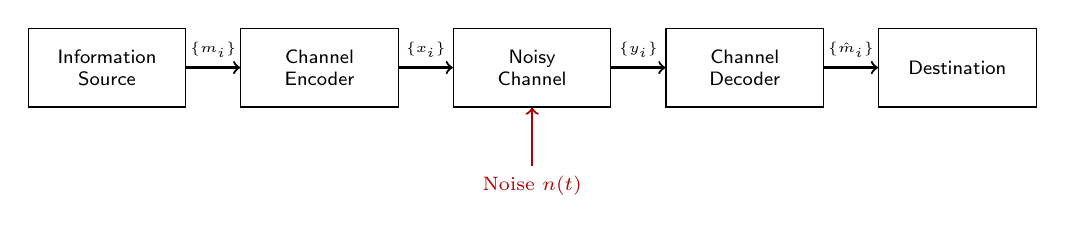
\begin{tikzpicture}[
  block/.style={rectangle, draw, minimum width=2cm, minimum height=1cm, font=\sffamily\scriptsize, align=center},
  node distance=2cm,
  font=\scriptsize
]
\node[block] (source) {Information\\Source};
\node[block, right of=source, node distance=2.7cm] (encoder) {Channel\\Encoder};
\node[block, right of=encoder, node distance=2.7cm] (channel) {Noisy\\Channel};
\node[block, right of=channel, node distance=2.7cm] (decoder) {Channel\\Decoder};
\node[block, right of=decoder, node distance=2.7cm] (dest) {Destination};

\draw[->,thick] (source) -- node[above,font=\tiny] {$\{m_i\}$} (encoder);
\draw[->,thick] (encoder) -- node[above,font=\tiny] {$\{x_i\}$} (channel);
\draw[->,thick] (channel) -- node[above,font=\tiny] {$\{y_i\}$} (decoder);
\draw[->,thick] (decoder) -- node[above,font=\tiny] {$\{\hat{m}_i\}$} (dest);

\node[below of=channel, node distance=1.5cm, font=\scriptsize, text=red!70!black] (noise) {Noise $n(t)$};
\draw[->,thick,red!70!black] (noise) -- (channel);
\end{tikzpicture}
\end{center}

\textbf{Key insight:} Shannon proved that by adding redundancy in the encoder (channel coding), we can approach arbitrarily low error rates at any data rate $R < C$.

\subsection{Capacity Region Visualization}

The relationship between data rate and reliability defines achievable performance:

\begin{center}
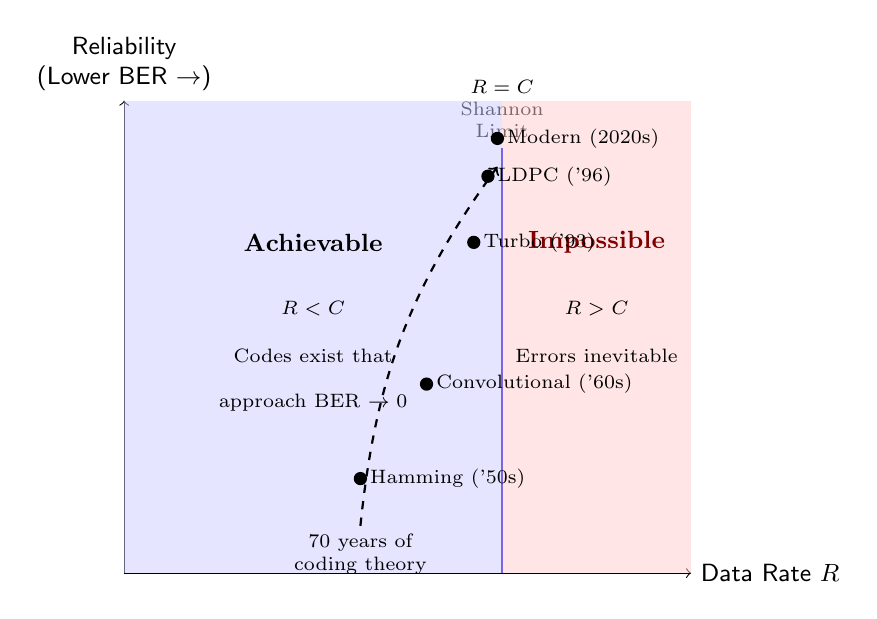
\begin{tikzpicture}[scale=1.2]
% Axes
\draw[->] (0,0) -- (6,0) node[right,font=\sffamily\small] {Data Rate $R$};
\draw[->] (0,0) -- (0,5) node[above,font=\sffamily\small,align=center] {Reliability\\(Lower BER $\rightarrow$)};

% Shannon capacity line
\draw[thick,blue] (4,0) -- (4,4.5) node[above,font=\scriptsize,text=black,align=center] {$R = C$\\Shannon\\Limit};

% Achievable region
\fill[blue!20,opacity=0.5] (0,0) rectangle (4,5);
\node[font=\small] at (2,3.5) {\textbf{Achievable}};
\node[font=\scriptsize] at (2,2.8) {$R < C$};
\node[font=\scriptsize] at (2,2.3) {Codes exist that};
\node[font=\scriptsize] at (2,1.8) {approach BER $\rightarrow 0$};

% Impossible region
\fill[red!20,opacity=0.5] (4,0) rectangle (6,5);
\node[font=\small,text=red!50!black] at (5,3.5) {\textbf{Impossible}};
\node[font=\scriptsize] at (5,2.8) {$R > C$};
\node[font=\scriptsize] at (5,2.3) {Errors inevitable};

% Practical codes markers
\fill[black] (2.5,1.0) circle (2pt) node[right,font=\scriptsize] {Hamming ('50s)};
\fill[black] (3.2,2.0) circle (2pt) node[right,font=\scriptsize] {Convolutional ('60s)};
\fill[black] (3.7,3.5) circle (2pt) node[right,font=\scriptsize] {Turbo ('93)};
\fill[black] (3.85,4.2) circle (2pt) node[right,font=\scriptsize] {LDPC ('96)};
\fill[black] (3.95,4.6) circle (2pt) node[right,font=\scriptsize] {Modern (2020s)};

% Arrow showing progress
\draw[->,thick,dashed] (2.5,0.5) to[bend left=15] (3.95,4.3);
\node[font=\scriptsize,align=center] at (2.5,0.2) {70 years of\\coding theory};

\end{tikzpicture}
\end{center}

\section{Performance Analysis}

\subsection{Capacity vs SNR Relationship}

The logarithmic relationship between capacity and SNR has profound implications:

\begin{center}
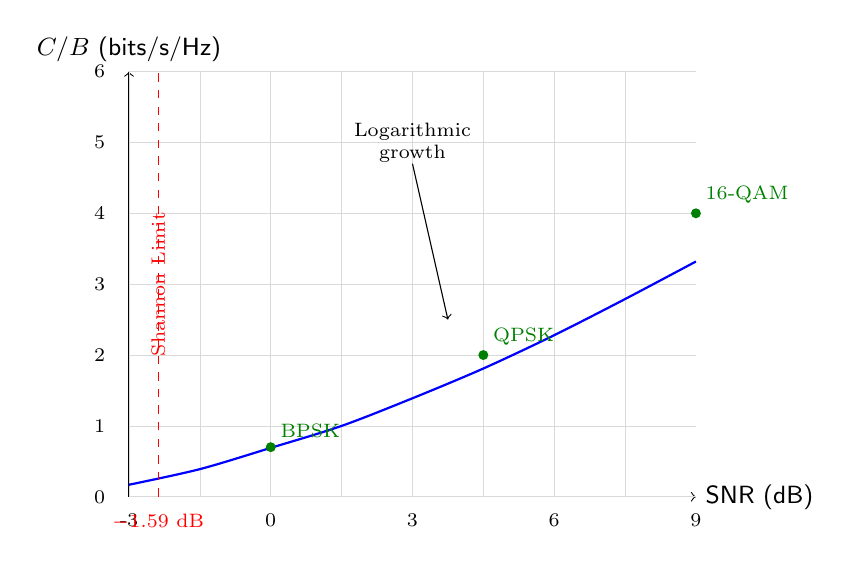
\begin{tikzpicture}[scale=0.9]
% Axes
\draw[->] (-2,0) -- (6,0) node[right,font=\sffamily\small] {SNR (dB)};
\draw[->] (-2,0) -- (-2,6) node[above,font=\sffamily\small] {$C/B$ (bits/s/Hz)};

% Grid
\foreach \x in {-2,-1,0,1,2,3,4,5}
  \draw[very thin,gray!30] (\x,0) -- (\x,6);
\foreach \y in {0,1,2,3,4,5,6}
  \draw[very thin,gray!30] (-2,\y) -- (6,\y);

% Axis labels
\foreach \x/\label in {-2/-3,0/0,2/3,4/6,6/9}
  \node[below,font=\scriptsize] at (\x,-0.1) {\label};
\foreach \y in {0,1,2,3,4,5,6}
  \node[left,font=\scriptsize] at (-2.2,\y) {\y};

% Shannon capacity curve: C/B = log2(1 + 10^(SNR_dB/10))
% Approximation points
\draw[thick,blue,smooth] plot coordinates {
  (-2,0.17) (-1,0.39) (0,0.69) (1,1.0) (2,1.39) (3,1.81) (4,2.28) (5,2.79) (6,3.32)
};

% Shannon limit annotation
\draw[dashed,red] (-1.59,0) -- (-1.59,6);
\node[rotate=90,font=\scriptsize,text=red] at (-1.59,3) {Shannon Limit};
\node[below,font=\scriptsize,text=red] at (-1.59,-0.1) {$-1.59$ dB};

% Practical modulation schemes
\fill[green!50!black] (0,0.7) circle (2pt) node[above right,font=\scriptsize] {BPSK};
\fill[green!50!black] (3,2.0) circle (2pt) node[above right,font=\scriptsize] {QPSK};
\fill[green!50!black] (6,4.0) circle (2pt) node[above right,font=\scriptsize] {16-QAM};

% Annotations
\node[font=\scriptsize,align=center] at (2,5) {Logarithmic\\growth};
\draw[->,thin] (2,4.7) -- (2.5,2.5);

\end{tikzpicture}
\end{center}

\begin{calloutbox}{Key Observation}
At low SNR (power-limited regime), capacity grows \textbf{linearly} with SNR: $C \approx B \cdot \mathrm{SNR} / \ln(2)$ for $\mathrm{SNR} \ll 1$.

At high SNR (bandwidth-limited regime), capacity grows \textbf{logarithmically}: $C \approx B \log_2(\mathrm{SNR})$ for $\mathrm{SNR} \gg 1$.

This explains why adding power becomes less effective as SNR increases---you need exponentially more power for linear capacity gains.
\end{calloutbox}

\subsection{Worked Examples}

\subsubsection{Example 1: WiFi Channel (802.11n)}

\textbf{Given:}
\begin{itemize}
\item Channel bandwidth: $B = 20$~MHz
\item Signal-to-noise ratio: $\mathrm{SNR} = 20$~dB $= 100$ (linear)
\end{itemize}

\textbf{Solution:}

Apply equation~\eqref{eq:shannon-capacity}:
\begin{align}
C &= B \log_2(1 + \mathrm{SNR}) \nonumber \\
  &= 20 \times 10^6 \cdot \log_2(1 + 100) \nonumber \\
  &= 20 \times 10^6 \cdot \log_2(101) \nonumber \\
  &= 20 \times 10^6 \cdot 6.66 \nonumber \\
  &= 133.2\,\text{Mbps}
\end{align}

Spectral efficiency:
\begin{equation}
\eta_{\max} = \frac{C}{B} = 6.66\,\text{bits/s/Hz}
\end{equation}

\textbf{Conclusion:} No matter how sophisticated the modulation or coding, this WiFi channel cannot reliably exceed 133~Mbps. Practical 802.11n systems achieve $\sim$100~Mbps (75\% of ca\-pac\-ity) using 64-QAM with rate-5/6 LDPC codes.

\subsubsection{Example 2: Deep Space Communication}

\textbf{Given:}
\begin{itemize}
\item Bandwidth: $B = 1$~MHz
\item Signal-to-noise ratio: $\mathrm{SNR} = -3$~dB $= 0.5$ (linear)
\end{itemize}

\textbf{Solution:}
\begin{align}
C &= 1 \times 10^6 \cdot \log_2(1 + 0.5) \nonumber \\
  &= 1 \times 10^6 \cdot \log_2(1.5) \nonumber \\
  &= 1 \times 10^6 \cdot 0.585 \nonumber \\
  &= 585\,\text{kbps}
\end{align}

\textbf{Key insight:} Even with \textbf{negative} SNR (noise power exceeds signal power), reliable communication is possible! The rate must be low, but Shannon's theorem guarantees codes exist that achieve near-zero error probability.

Voyager spacecraft operate near this regime using rate-1/6 convolutional codes with constraint length 15.

\subsubsection{Example 3: Extreme Low-SNR (Chimera-Like)}

\textbf{Scenario:} Underwater acoustic communication or covert RF link

\textbf{Given:}
\begin{itemize}
\item Bandwidth: $B = 20$~Hz (narrow-band)
\item SNR: $-15$~dB $= 0.0316$ (linear)
\item Modulation: QPSK (2 bits/symbol)
\item Symbol rate: $R_s = 10$~symbols/s
\end{itemize}

\textbf{Solution:}

Channel capacity:
\begin{align}
C &= 20 \cdot \log_2(1 + 0.0316) \nonumber \\
  &= 20 \cdot \log_2(1.0316) \nonumber \\
  &= 20 \cdot 0.045 \nonumber \\
  &= 0.9\,\text{bps}
\end{align}

Raw data rate without FEC:
\begin{equation}
R_{\text{raw}} = R_s \times \log_2(M) = 10 \times 2 = 20\,\text{bps}
\end{equation}

Rate ratio:
\begin{equation}
\frac{R_{\text{raw}}}{C} = \frac{20}{0.9} = 22.2 \gg 1
\end{equation}

\textbf{Analysis:} Operating 22$\times$ above capacity is impossible without FEC!

With rate-1/2 LDPC code:
\begin{equation}
R_{\text{coded}} = 20 \times 0.5 = 10\,\text{bps}, \quad \frac{R_{\text{coded}}}{C} = 11.1
\end{equation}

Still operating above capacity! A rate-1/20 code or higher bandwidth/SNR is needed.

\begin{warningbox}
This example illustrates why extremely low-SNR links require \textbf{massive error correction overhead}. A rate-1/20 code means sending 20 parity bits for every 1 information bit---but this is the price Shannon's theorem demands for reliable communication in extreme noise.
\end{warningbox}

\section{Spectral Efficiency Analysis}

\subsection{Maximum Spectral Efficiency}

From equation~\eqref{eq:spectral-efficiency}, the maximum achievable spectral efficiency is:
\begin{equation}
\eta_{\max} = \log_2(1 + \mathrm{SNR}) \quad \text{bits/s/Hz}
\end{equation}

\textbf{Benchmark values:}

\begin{center}
\begin{tabular}{@{}rrr@{}}
\toprule
SNR (linear) & SNR (dB) & $\eta_{\max}$ (bits/s/Hz) \\
\midrule
1 & 0 & 1.0 \\
3 & 4.8 & 2.0 \\
7 & 8.5 & 3.0 \\
15 & 11.8 & 4.0 \\
31 & 14.9 & 5.0 \\
63 & 18.0 & 6.0 \\
255 & 24.1 & 8.0 \\
1023 & 30.1 & 10.0 \\
\bottomrule
\end{tabular}
\end{center}

\textbf{Key insight:} Each doubling of spectral efficiency requires approximately \textbf{6~dB more SNR} (4$\times$ signal power or 1/4 the noise).

\subsection{Practical System Performance}

Real communication systems operate below Shannon's limit due to practical constraints:

\begin{center}
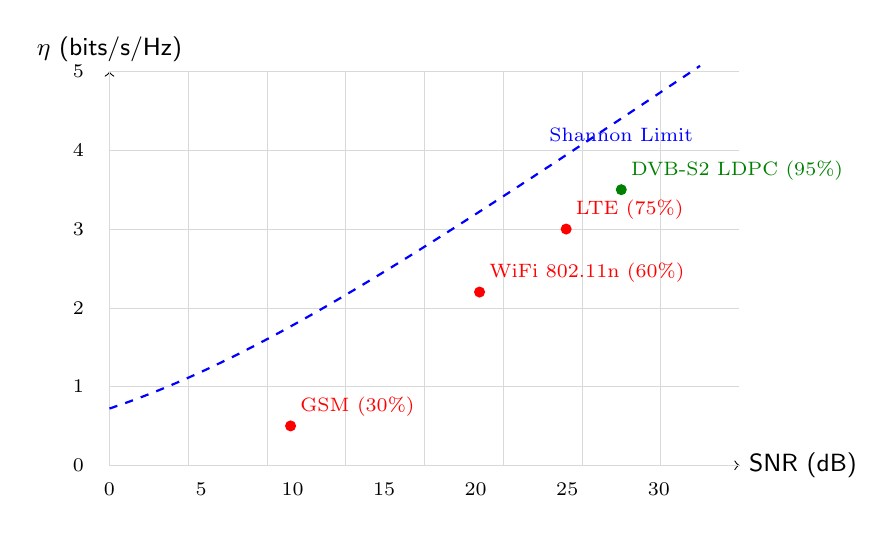
\begin{tikzpicture}[scale=1.0]
% Axes
\draw[->] (0,0) -- (8,0) node[right,font=\sffamily\small] {SNR (dB)};
\draw[->] (0,0) -- (0,5) node[above,font=\sffamily\small] {$\eta$ (bits/s/Hz)};

% Grid
\foreach \x in {0,1,...,7}
  \draw[very thin,gray!30] (\x,0) -- (\x,5);
\foreach \y in {0,1,2,3,4,5}
  \draw[very thin,gray!30] (0,\y) -- (8,\y);

% Axis labels
\foreach \x in {0,5,10,15,20,25,30}
  \node[below,font=\scriptsize] at (\x/4.3,-0.1) {\x};
\foreach \y in {0,1,2,3,4,5}
  \node[left,font=\scriptsize] at (-0.2,\y) {\y};

% Shannon limit curve
\draw[thick,blue,dashed] plot[smooth,domain=0:7.5] (\x,{0.72*ln(1+exp(\x*0.65))/ln(2)});
\node[blue,font=\scriptsize] at (6.5,4.2) {Shannon Limit};

% Practical systems
\fill[red] (2.3,0.5) circle (2pt) node[above right,font=\scriptsize] {GSM (30\%)};
\fill[red] (4.7,2.2) circle (2pt) node[above right,font=\scriptsize] {WiFi 802.11n (60\%)};
\fill[red] (5.8,3.0) circle (2pt) node[above right,font=\scriptsize] {LTE (75\%)};
\fill[green!50!black] (6.5,3.5) circle (2pt) node[above right,font=\scriptsize] {DVB-S2 LDPC (95\%)};

\end{tikzpicture}
\end{center}

\textbf{Efficiency comparison:}

\begin{center}
\begin{tabular}{@{}lrrr@{}}
\toprule
System & Typical SNR & $\eta$ Achieved & \% of Shannon \\
\midrule
GSM & 10~dB & 0.5 & 30\% \\
WiFi 802.11n & 20~dB & 3.5 & 60\% \\
LTE Advanced & 25~dB & 5.0 & 75\% \\
5G NR & 30~dB & 7.5 & 90\% \\
DVB-S2 (LDPC) & Variable & Adaptive & 95\% \\
\bottomrule
\end{tabular}
\end{center}

\begin{keyconcept}
Modern error-correction codes (LDPC, Turbo, Polar) achieve \textbf{$>$95\% of Shannon capacity}. After 70 years of coding theory research, we have effectively ``solved'' Shannon's challenge for AWGN channels.

The remaining gap to 100\% requires exponentially increasing decoder complexity---the final few tenths of a dB are not economically justified for most applications.
\end{keyconcept}

\section{Power-Limited vs Bandwidth-Limited Regimes}

Shannon's capacity formula behaves differently in low-SNR and high-SNR scenarios, leading to fundamentally different system design strategies.

\subsection{Power-Limited Regime (Low SNR)}

When $\mathrm{SNR} \ll 1$ (satellite, deep space, underwater acoustic), approximate equation~\eqref{eq:shannon-capacity} using $\ln(1+x) \approx x$:
\begin{equation}
C \approx B \cdot \frac{\mathrm{SNR}}{\ln(2)} \approx 1.443 \cdot B \cdot \mathrm{SNR} \quad \text{(for SNR $\ll$ 1)}
\label{eq:power-limited}
\end{equation}

\textbf{Capacity grows linearly with power}, making every dB of transmit power valuable.

\textbf{Design strategy:}
\begin{itemize}
\item Use \textbf{low spectral efficiency} ($\eta \ll 1$~bits/s/Hz)
\item Apply \textbf{strong FEC} (rate 1/4, 1/6, even 1/20)
\item \textbf{Spread spectrum} techniques to increase processing gain
\item Simple modulation (BPSK, QPSK) for power efficiency
\end{itemize}

\textbf{Example systems:}
\begin{itemize}
\item Voyager 1/2: Rate-1/6 convolutional code, BPSK, $E_b/N_0 \approx 2$~dB
\item GPS: BPSK with spreading gain 43~dB
\item Deep-space links: $\mathrm{SNR} = -20$ to $-10$~dB common
\end{itemize}

\subsection{Bandwidth-Limited Regime (High SNR)}

When $\mathrm{SNR} \gg 1$ (fiber optics, microwave backhaul), equation~\eqref{eq:shannon-capacity} simplifies:
\begin{equation}
C \approx B \log_2(\mathrm{SNR}) \quad \text{(for SNR $\gg$ 1)}
\label{eq:bandwidth-limited}
\end{equation}

\textbf{Capacity grows logarithmically with power}---dou\-bling ca\-pac\-ity requires squaring SNR (6~dB).

\textbf{Design strategy:}
\begin{itemize}
\item Use \textbf{high spectral efficiency} ($\eta \approx 6$--10~bits/s/Hz)
\item High-order modulation (64-QAM, 256-QAM, 1024-QAM)
\item \textbf{Light FEC} (rate 8/9, 9/10) to minimize overhead
\item Multiple antennas (MIMO) to increase effective bandwidth
\end{itemize}

\textbf{Example systems:}
\begin{itemize}
\item Fiber optics: 256-QAM, SNR $>$ 35~dB, rate-0.95 codes
\item 5G mmWave: 256-QAM, LDPC rate 8/9
\item Cable modems (DOCSIS 3.1): 4096-QAM in clean channels
\end{itemize}

\subsection{Trade-Off Visualization}

\begin{center}
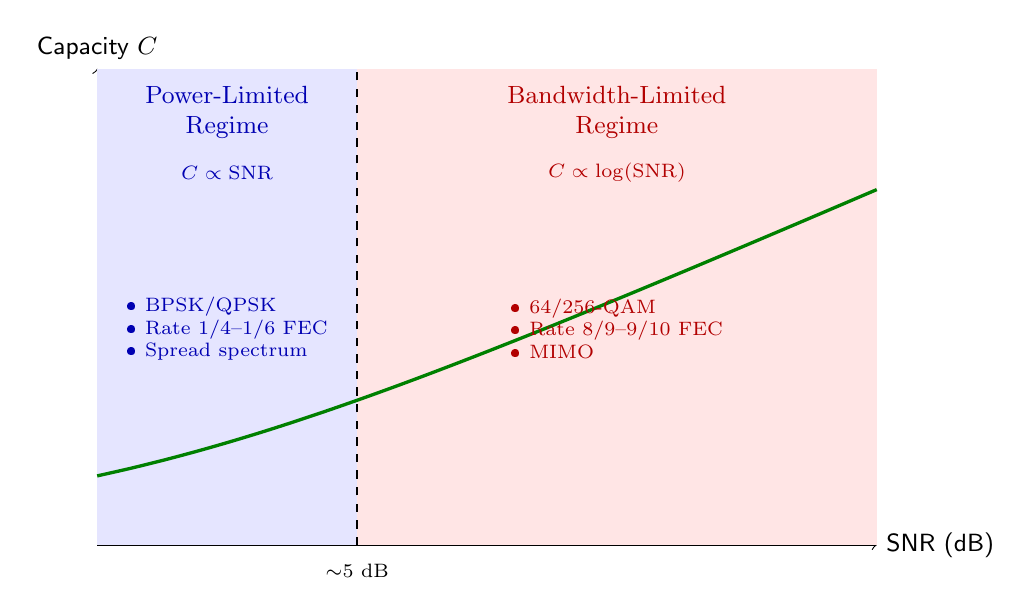
\begin{tikzpicture}[scale=1.1]
% Axes
\draw[->] (0,0) -- (9,0) node[right,font=\sffamily\small] {SNR (dB)};
\draw[->] (0,0) -- (0,5.5) node[above,font=\sffamily\small] {Capacity $C$};

% Two regions
\fill[blue!10] (0,0) rectangle (3,5.5);
\fill[red!10] (3,0) rectangle (9,5.5);

\node[font=\small,text=blue!70!black,align=center] at (1.5,5) {Power-Limited\\Regime};
\node[font=\scriptsize,text=blue!70!black] at (1.5,4.3) {$C \propto \mathrm{SNR}$};

\node[font=\small,text=red!70!black,align=center] at (6,5) {Bandwidth-Limited\\Regime};
\node[font=\scriptsize,text=red!70!black] at (6,4.3) {$C \propto \log(\mathrm{SNR})$};

% Capacity curve (schematic)
\draw[very thick,green!50!black] plot[smooth,domain=0:9] (\x,{0.6*ln(1+exp(\x*0.5))/ln(2)+0.2});

% Design strategies
\node[font=\scriptsize,align=left,text=blue!70!black] at (1.5,2.5) {
  • BPSK/QPSK\\
  • Rate 1/4--1/6 FEC\\
  • Spread spectrum
};

\node[font=\scriptsize,align=left,text=red!70!black] at (6,2.5) {
  • 64/256-QAM\\
  • Rate 8/9--9/10 FEC\\
  • MIMO
};

% Transition line
\draw[dashed,thick] (3,0) -- (3,5.5);
\node[below,font=\scriptsize] at (3,-0.1) {$\sim$5 dB};

\end{tikzpicture}
\end{center}

\begin{calloutbox}{Practical Implication}
Satellite engineers fight for every 0.1~dB of $E_b/N_0$ (power-limited), while fiber-optic engineers care more about maximizing bits/s/Hz (bandwidth-limited).

Shannon's theorem explains this dichotomy: the same capacity formula yields opposite design priorities depending on the operating SNR.
\end{calloutbox}

\section{Historical Context}

\subsection{Shannon's Original Theorem (1948)}

The original Shannon-Hartley formula:
\begin{equation}
C = B \log_2\left(1 + \frac{S}{N}\right)
\end{equation}
where $S$ and $N$ are signal and noise \textbf{power} (not ratios).

\textbf{Key assumptions:}
\begin{enumerate}
\item AWGN channel (additive white Gaussian noise)
\item Average power constraint on transmitter
\item Unlimited complexity allowed for encoder/decoder
\item Infinite delay acceptable (arbitrarily long block codes)
\end{enumerate}

\textbf{What Shannon did NOT provide:}
\begin{itemize}
\item How to construct codes achieving capacity
\item Practical complexity or delay bounds
\item Performance at finite block length
\end{itemize}

Shannon proved codes \textit{exist} but left their construction ``as an exercise for humanity.''

\subsection{70 Years of Progress}

\begin{center}
\begin{tabular}{@{}lll@{}}
\toprule
Year & Code Type & Gap to Shannon Limit \\
\midrule
1948 & \textbf{Shannon proves limit} & Baseline established \\
1950 & Hamming codes & $\sim$7~dB \\
1955 & BCH codes & $\sim$5~dB \\
1960 & Convolutional codes & $\sim$3~dB \\
1974 & Concatenated codes & $\sim$2~dB \\
1993 & \textbf{Turbo codes} & $\sim$0.7~dB (breakthrough!) \\
1996 & \textbf{LDPC rediscovered} & $\sim$0.5~dB \\
2008 & \textbf{Polar codes} & $\sim$0.5~dB \\
2020 & Modern LDPC (DVB-S2X) & $\sim$0.2~dB \\
\bottomrule
\end{tabular}
\end{center}

\begin{calloutbox}{Remarkable Achievement}
It took 45 years (1948--1993) to get within 1~dB of Shannon's limit. Turbo codes, announced in 1993, shocked the coding community by achieving 0.7~dB. Modern codes are now within 0.2~dB---we have essentially ``solved'' Shannon's challenge for AWGN channels.

The remaining gap requires exponentially increasing complexity and is not economically justified for most applications.
\end{calloutbox}

\section{The BER Waterfall Effect}

Capacity-approaching codes exhibit a distinctive ``waterfall'' behavior in BER performance:

\begin{center}
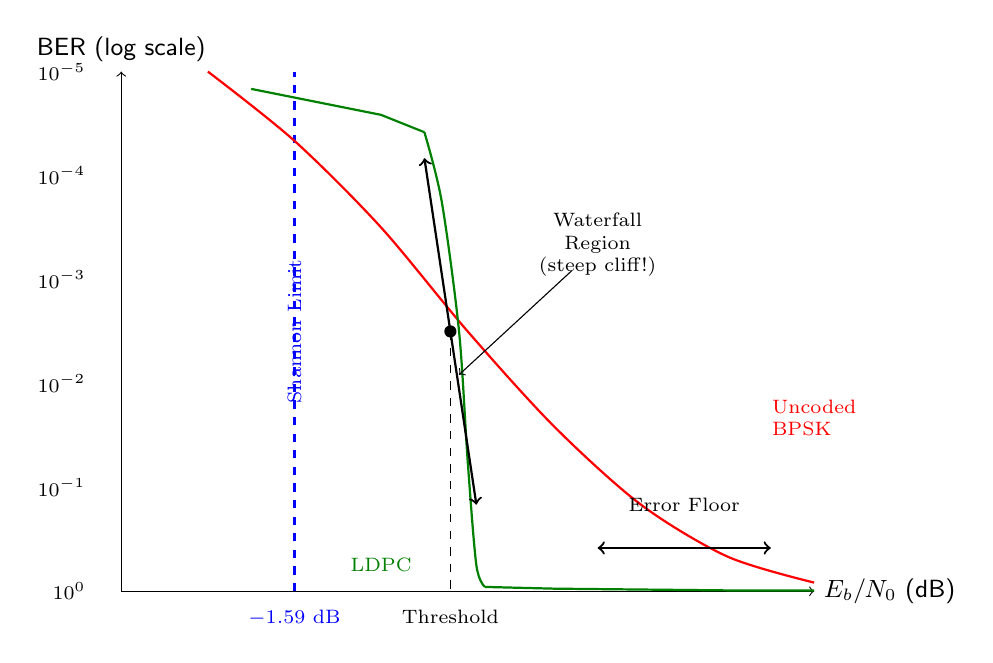
\begin{tikzpicture}[scale=1.1]
% Axes (log scale for BER)
\draw[->] (0,0) -- (8,0) node[right,font=\sffamily\small] {$E_b/N_0$ (dB)};
\draw[->] (0,0) -- (0,6) node[above,font=\sffamily\small] {BER (log scale)};

% Y-axis labels (log scale)
\foreach \y/\label in {0/10^0,1/10^{-1},2/10^{-2},3/10^{-3},4/10^{-4},5/10^{-5}}
  \node[left,font=\scriptsize] at (-0.3,\y*1.2) {$\label$};

% Shannon limit line
\draw[thick,dashed,blue] (2,0) -- (2,6);
\node[rotate=90,font=\scriptsize,blue] at (2,3) {Shannon Limit};
\node[below,font=\scriptsize,blue] at (2,-0.1) {$-1.59$ dB};

% Uncoded BPSK (smooth curve)
\draw[thick,red,smooth] plot coordinates {
  (1,6) (2,5.2) (3,4.2) (4,3.0) (5,1.9) (6,1.0) (7,0.4) (8,0.1)
};
\node[red,font=\scriptsize,align=left] at (8,2) {Uncoded\\BPSK};

% LDPC waterfall
\draw[thick,green!50!black] plot coordinates {
  (1.5,5.8) (2.5,5.6) (3.0,5.5) (3.5,5.3)
};
\draw[thick,green!50!black,smooth] plot coordinates {
  (3.5,5.3) (3.7,4.5) (3.9,3.0) (4.0,1.5) (4.1,0.3) (4.2,0.05)
};
\draw[thick,green!50!black] plot coordinates {
  (4.2,0.05) (5,0.03) (6,0.02) (7,0.01) (8,0.01)
};

% Waterfall annotation
\draw[<->,thick] (3.5,5.0) -- (4.1,1.0);
\node[font=\scriptsize,align=center] at (5.5,4) {Waterfall\\Region\\(steep cliff!)};
\draw[->,thin] (5.2,3.7) -- (3.9,2.5);

% Floor annotation
\draw[<->,thick] (5.5,0.5) -- (7.5,0.5);
\node[font=\scriptsize,align=center] at (6.5,1.0) {Error Floor};

\node[green!50!black,font=\scriptsize] at (3,0.3) {LDPC};

% Threshold point
\fill[black] (3.8,3.0) circle (2pt);
\draw[dashed,thin] (3.8,3.0) -- (3.8,0);
\node[below,font=\scriptsize] at (3.8,-0.1) {Threshold};

\end{tikzpicture}
\end{center}

\subsection{Three Regions of Performance}

\subsubsection{1. Pre-Waterfall Region ($E_b/N_0 < $ Threshold)}

\begin{itemize}
\item BER remains high ($>10^{-3}$)
\item Code cannot reliably correct errors
\item Decoder iterations fail to converge
\item Small SNR improvements yield minimal BER reduction
\end{itemize}

\subsubsection{2. Waterfall Region (Near Threshold)}

\begin{itemize}
\item \textbf{Dramatic BER improvement} (3--5 orders of magnitude drop)
\item Occurs over narrow SNR range (0.5--1.5~dB)
\item Code begins effective error correction
\item Characteristic of capacity-approaching codes
\end{itemize}

For LDPC codes, the waterfall typically occurs at $E_b/N_0 \approx $ Shannon limit $+ 0.5$~dB.

\subsubsection{3. Error Floor ($E_b/N_0 > $ Threshold + 2~dB)}

\begin{itemize}
\item BER levels off at constant value ($10^{-5}$ to $10^{-8}$)
\item Caused by decoder sub-optimal performance
\item Due to problematic code structures (trapping sets, stopping sets)
\item Further SNR increases yield little BER improvement
\end{itemize}

\begin{warningbox}
\textbf{Error floors are a practical limitation of capacity-approaching codes.}

For applications requiring BER $< 10^{-10}$ (e.g., optical fiber), outer codes (BCH, RS) are concatenated to ``break through'' the floor. The trade-off is added latency and complexity.
\end{warningbox}

\subsection{Practical Threshold Definition}

The \textbf{threshold} $E_b/N_0$ is typically defined as the SNR where:
\begin{equation}
\mathrm{BER} = 10^{-5} \quad \text{or} \quad 10^{-6}
\end{equation}

This represents the boundary between unreliable and reliable operation for most practical systems.

\section{Applications in Modern Systems}

Shannon's capacity theorem directly guides the design of all modern communication systems.

\subsection{Adaptive Modulation and Coding (AMC)}

Modern wireless systems (LTE, 5G, WiFi 6) dynamically adjust modulation and coding to track channel capacity in real-time.

\subsubsection{AMC Algorithm}

\textbf{Process:}
\begin{enumerate}
\item Receiver estimates instantaneous SNR
\item Compute available capacity: $C = B \log_2(1 + \mathrm{SNR})$
\item Select modulation and code rate such that $R < C$ with safety margin
\item Feedback MCS (Modulation-Coding Scheme) index to transmitter
\item Transmitter adjusts parameters for next frame
\end{enumerate}

\textbf{MCS Table Example (LTE):}

\begin{center}
\begin{tabular}{@{}lrrr@{}}
\toprule
MCS & Modulation & Code Rate & Spectral Eff. (bits/s/Hz) \\
\midrule
0 & QPSK & 1/5 & 0.4 \\
5 & QPSK & 1/2 & 1.0 \\
10 & 16-QAM & 1/2 & 2.0 \\
15 & 64-QAM & 2/3 & 4.0 \\
20 & 256-QAM & 3/4 & 6.0 \\
28 & 256-QAM & 9/10 & 7.2 \\
\bottomrule
\end{tabular}
\end{center}

Each MCS is designed to operate reliably at a specific SNR range, always staying below Shannon capacity.

\subsection{Satellite Communication (DVB-S2)}

Digital Video Broadcasting Satellite (DVB-S2) uses 28 different modulation-coding combinations:

\begin{calloutbox}[colback=black!5!white,colframe=black]{DVB-S2 System}
\textbf{Parameters:}
\begin{itemize}
\item Modulation: QPSK, 8PSK, 16-APSK, 32-APSK
\item Code rates: 1/4, 1/3, 2/5, 1/2, 3/5, 2/3, 3/4, 4/5, 5/6, 8/9, 9/10
\item FEC: LDPC + BCH outer code
\item Efficiency: 0.5 to 5.0 bits/s/Hz
\end{itemize}

\textbf{Performance:} Operates within 0.6--0.8~dB of Shannon limit across all modes.
\end{calloutbox}

\subsection{Deep-Space Communication}

NASA Deep Space Network illustrates power-limited design:

\textbf{Mars Reconnaissance Orbiter (MRO):}
\begin{itemize}
\item Distance: $\sim$225 million km (at conjunction)
\item Transmit power: 100~W
\item Frequency: X-band (8.4~GHz)
\item Data rate: 0.5--6~Mbps (adaptive)
\item Modulation: BPSK, QPSK
\item Coding: Turbo code (rate 1/6 to 6/7)
\item Performance: $E_b/N_0 \approx 2$--4~dB (near Shannon limit)
\end{itemize}

\subsection{5G New Radio}

5G NR exploits Shannon's theorem through:

\begin{enumerate}
\item \textbf{Massive MIMO:} 64--256 antennas multiply effective capacity
\item \textbf{mmWave spectrum:} Bandwidth $B$ up to 400~MHz (increases $C$)
\item \textbf{LDPC codes:} Rate 1/5 to 8/9, within 0.5~dB of Shannon
\item \textbf{256-QAM:} High spectral efficiency in good channels
\end{enumerate}

Result: Peak data rates exceeding 10~Gbps (comparable to fiber).

\subsection{Underwater Acoustic Communication}

Extreme power-limited regime:

\begin{itemize}
\item Typical SNR: $-10$ to $+10$~dB
\item Bandwidth: 1--50~kHz (severely limited)
\item Capacity: Few hundred bits/s to few kbps
\item Design: QPSK, rate-1/2 convolutional codes, multi-carrier
\item Challenge: Multipath + Doppler + low SNR simultaneously
\end{itemize}

\begin{calloutbox}{Key Lesson}
Every successful communication system operates \textbf{within} Shannon's capacity bound. The theorem doesn't tell you \textit{how} to build the system---but it tells you what's \textit{impossible}, preventing engineers from chasing unattainable performance goals.
\end{calloutbox}

\section{Extensions and Generalizations}

\subsection{Fading Channels}

For Rayleigh fading channels, capacity is reduced compared to AWGN:
\begin{equation}
C_{\text{fading}} = B \cdot \mathbb{E}\left[\log_2(1 + \gamma \cdot \mathrm{SNR})\right]
\end{equation}
where $\gamma$ is the random fading coefficient and $\mathbb{E}[\cdot]$ denotes expectation.

\textbf{Mitigation strategies:}
\begin{itemize}
\item \textbf{Diversity:} Spatial (antennas), temporal (interleaving), spectral (OFDM)
\item \textbf{Channel coding + interleaving:} Spread errors across multiple fading realizations
\item \textbf{Adaptive modulation:} Exploit good channel states, back off during deep fades
\end{itemize}

\subsection{MIMO Channels}

With $N_T$ transmit and $N_R$ receive antennas:
\begin{equation}
C_{\text{MIMO}} \approx \min(N_T, N_R) \cdot B \log_2(1 + \mathrm{SNR})
\end{equation}

\textbf{Capacity grows linearly with number of spatial streams!}

This fundamental result drives massive MIMO in 5G (64--256 antennas), achieving capacities exceeding 100~bits/s/Hz in favorable conditions.

\subsection{Non-Gaussian Noise}

Shannon's theorem assumes Gaussian noise (worst-case for given variance). For other noise distributions:
\begin{itemize}
\item \textbf{Impulsive noise:} Capacity can be higher (noise concentrated in time)
\item \textbf{Colored noise:} Pre-whitening filter restores AWGN model
\item \textbf{Interference:} Capacity depends on interference structure (can be treated as noise or decoded)
\end{itemize}

\section{Information-Theoretic Foundation}

\subsection{Mutual Information}

The capacity formula derives from \textbf{mutual information} $I(X;Y)$:
\begin{equation}
I(X;Y) = H(Y) - H(Y|X)
\end{equation}
where:
\begin{itemize}
\item $H(Y)$ = entropy of received signal (total uncertainty)
\item $H(Y|X)$ = conditional entropy (uncertainty due to noise)
\item $I(X;Y)$ = information transmitted from $X$ to $Y$
\end{itemize}

\subsection{Capacity Definition}

Channel capacity is the maximum mutual information over all input distributions:
\begin{equation}
C = \max_{p(x)} I(X;Y)
\label{eq:capacity-definition}
\end{equation}

For the AWGN channel, the optimal input distribution is \textbf{Gaussian} with power constraint $P_s$, yielding:
\begin{equation}
C = B \log_2\left(1 + \frac{P_s}{N_0 B}\right)
\end{equation}

This result is remarkable: the capacity depends only on bandwidth, signal power, and noise power---independent of modulation scheme or coding technique.

\section{Summary}

Shannon's Channel Capacity Theorem is the cornerstone of modern communication theory.

\subsection{Key Principles}

\begin{enumerate}
\item \textbf{Fundamental Limit:} $C = B \log_2(1 + \mathrm{SNR})$ is an absolute bound. No system can exceed this rate reliably.

\item \textbf{Achievability:} For any rate $R < C$, codes exist that achieve arbitrarily low error probability. Shannon proved existence without construction.

\item \textbf{Converse:} For $R > C$, reliable communication is impossible regardless of coding complexity.

\item \textbf{Power-Bandwidth Trade-off:} Capacity can be maintained by exchanging bandwidth for power, or vice versa. Spread spectrum exploits this principle.

\item \textbf{Modern Achievement:} LDPC, Turbo, and Polar codes operate within 0.2--0.5~dB of Shannon's limit---we have essentially ``solved'' the AWGN channel.

\item \textbf{Design Guidance:} All practical systems must satisfy $R < C$. Adaptive modulation and coding dynamically track capacity as channel conditions vary.
\end{enumerate}

\subsection{Historical Impact}

Shannon's 1948 paper revolutionized communication engineering:
\begin{itemize}
\item \textbf{Before Shannon:} Engineers believed noise fundamentally limited reliability
\item \textbf{Shannon's insight:} Error-free communication is possible below capacity using coding
\item \textbf{After Shannon:} 70 years of coding theory research to approach the limit
\item \textbf{Today:} Capacity-approaching codes (LDPC, Turbo) are deployed in billions of devices
\end{itemize}

\begin{keyconcept}
Shannon's theorem doesn't tell you \textit{how} to build a communication system---but it tells you what's \textit{possible} and what's \textit{impossible}. This boundary between achievable and unachievable is the most fundamental result in information theory.
\end{keyconcept}

\subsection{Cross-References}

\begin{itemize}
\item Chapter~\ref{ch:ber}: Bit Error Rate (BER) - Performance metric
\item Chapter~\ref{ch:awgn}: AWGN Channel - Where Shannon's formula applies
\item Forward Error Correction (FEC) - Methods to approach Shannon limit
\item LDPC Codes - Modern capacity-approaching codes
\item Energy Ratios ($E_b/N_0$) - Alternative formulation of SNR
\item Signal-to-Noise Ratio (SNR) - Key parameter in capacity formula
\end{itemize}

\section{References}

\subsection{Primary Sources}

\begin{enumerate}
\item \textbf{Shannon, C.E.} (1948) ``A Mathematical Theory of Communication'' \textit{Bell System Technical Journal} 27, 379--423, 623--656
  \begin{itemize}
  \item The foundational paper---remarkably accessible and still highly readable today
  \end{itemize}

\item \textbf{Shannon, C.E.} (1949) ``Communication in the Presence of Noise'' \textit{Proceedings of the IRE} 37, 10--21
  \begin{itemize}
  \item Shannon-Hartley theorem for AWGN channels
  \item Introduces the sampling theorem
  \end{itemize}
\end{enumerate}

\subsection{Textbooks}

\begin{enumerate}
\setcounter{enumi}{2}
\item \textbf{Cover, T.M. \& Thomas, J.A.} (2006) \textit{Elements of Information Theory}, 2nd ed. (Wiley)
  \begin{itemize}
  \item Definitive graduate-level textbook
  \item Comprehensive coverage of Shannon theory
  \end{itemize}

\item \textbf{MacKay, D.J.C.} (2003) \textit{Information Theory, Inference, and Learning Algorithms} (Cambridge University Press)
  \begin{itemize}
  \item Free online at \texttt{www.inference.org.uk/mackay/itila/}
  \item Excellent intuitive explanations
  \end{itemize}

\item \textbf{Gallager, R.G.} (1968) \textit{Information Theory and Reliable Communication} (Wiley)
  \begin{itemize}
  \item Classic text by LDPC code inventor
  \item Rigorous mathematical treatment
  \end{itemize}
\end{enumerate}

\subsection{Historical Perspectives}

\begin{enumerate}
\setcounter{enumi}{5}
\item \textbf{Verdú, S.} (1998) ``Fifty Years of Shannon Theory'' \textit{IEEE Transactions on Information Theory} 44(6), 2057--2078
  \begin{itemize}
  \item Comprehensive review of progress since 1948
  \item Survey of modern coding techniques
  \end{itemize}

\item \textbf{Berrou, C., Glavieux, A., \& Thitimajshima, P.} (1993) ``Near Shannon Limit Error-Correcting Coding and Decoding: Turbo-Codes'' \textit{Proc. IEEE ICC}
  \begin{itemize}
  \item Breakthrough paper introducing Turbo codes
  \item First practical codes within 1~dB of Shannon limit
  \end{itemize}
\end{enumerate}
